%% matter tex
%% begins with section

\begin{frame}
\begin{center}
\vspace*{\vfill}
{\Large F}ast \hfill $\sim$ milli-second\\
{\Large R}adio \hfill $\sim$ radio-regime \emph{???}\\
{\Large B}urst \hfill $\sim$ Like an explosion\\
\begin{figure}
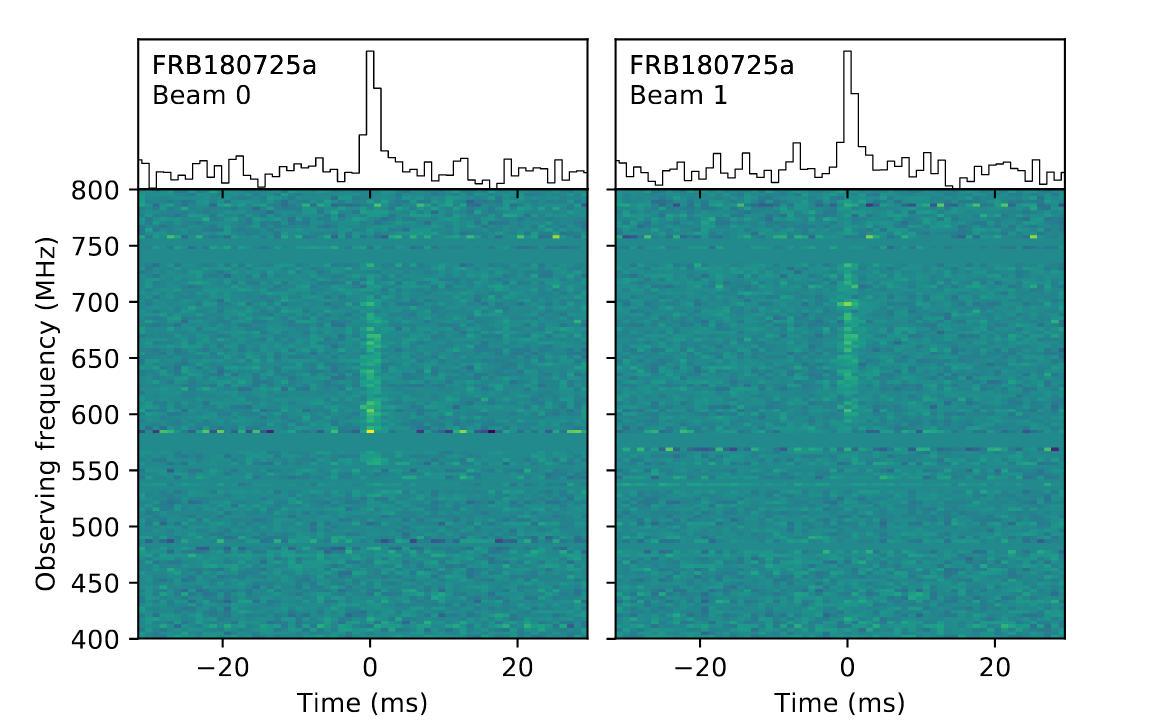
\includegraphics[width=\textwidth, keepaspectratio]{frbdef.png}
\caption{ATel\#11901:First CHIME/FRB detection at 400-800 MHz}
\end{figure}
\vspace*{\vfill}
\end{center}
\end{frame}

% \begin{frame}
% \begin{figure}
% \centering
% 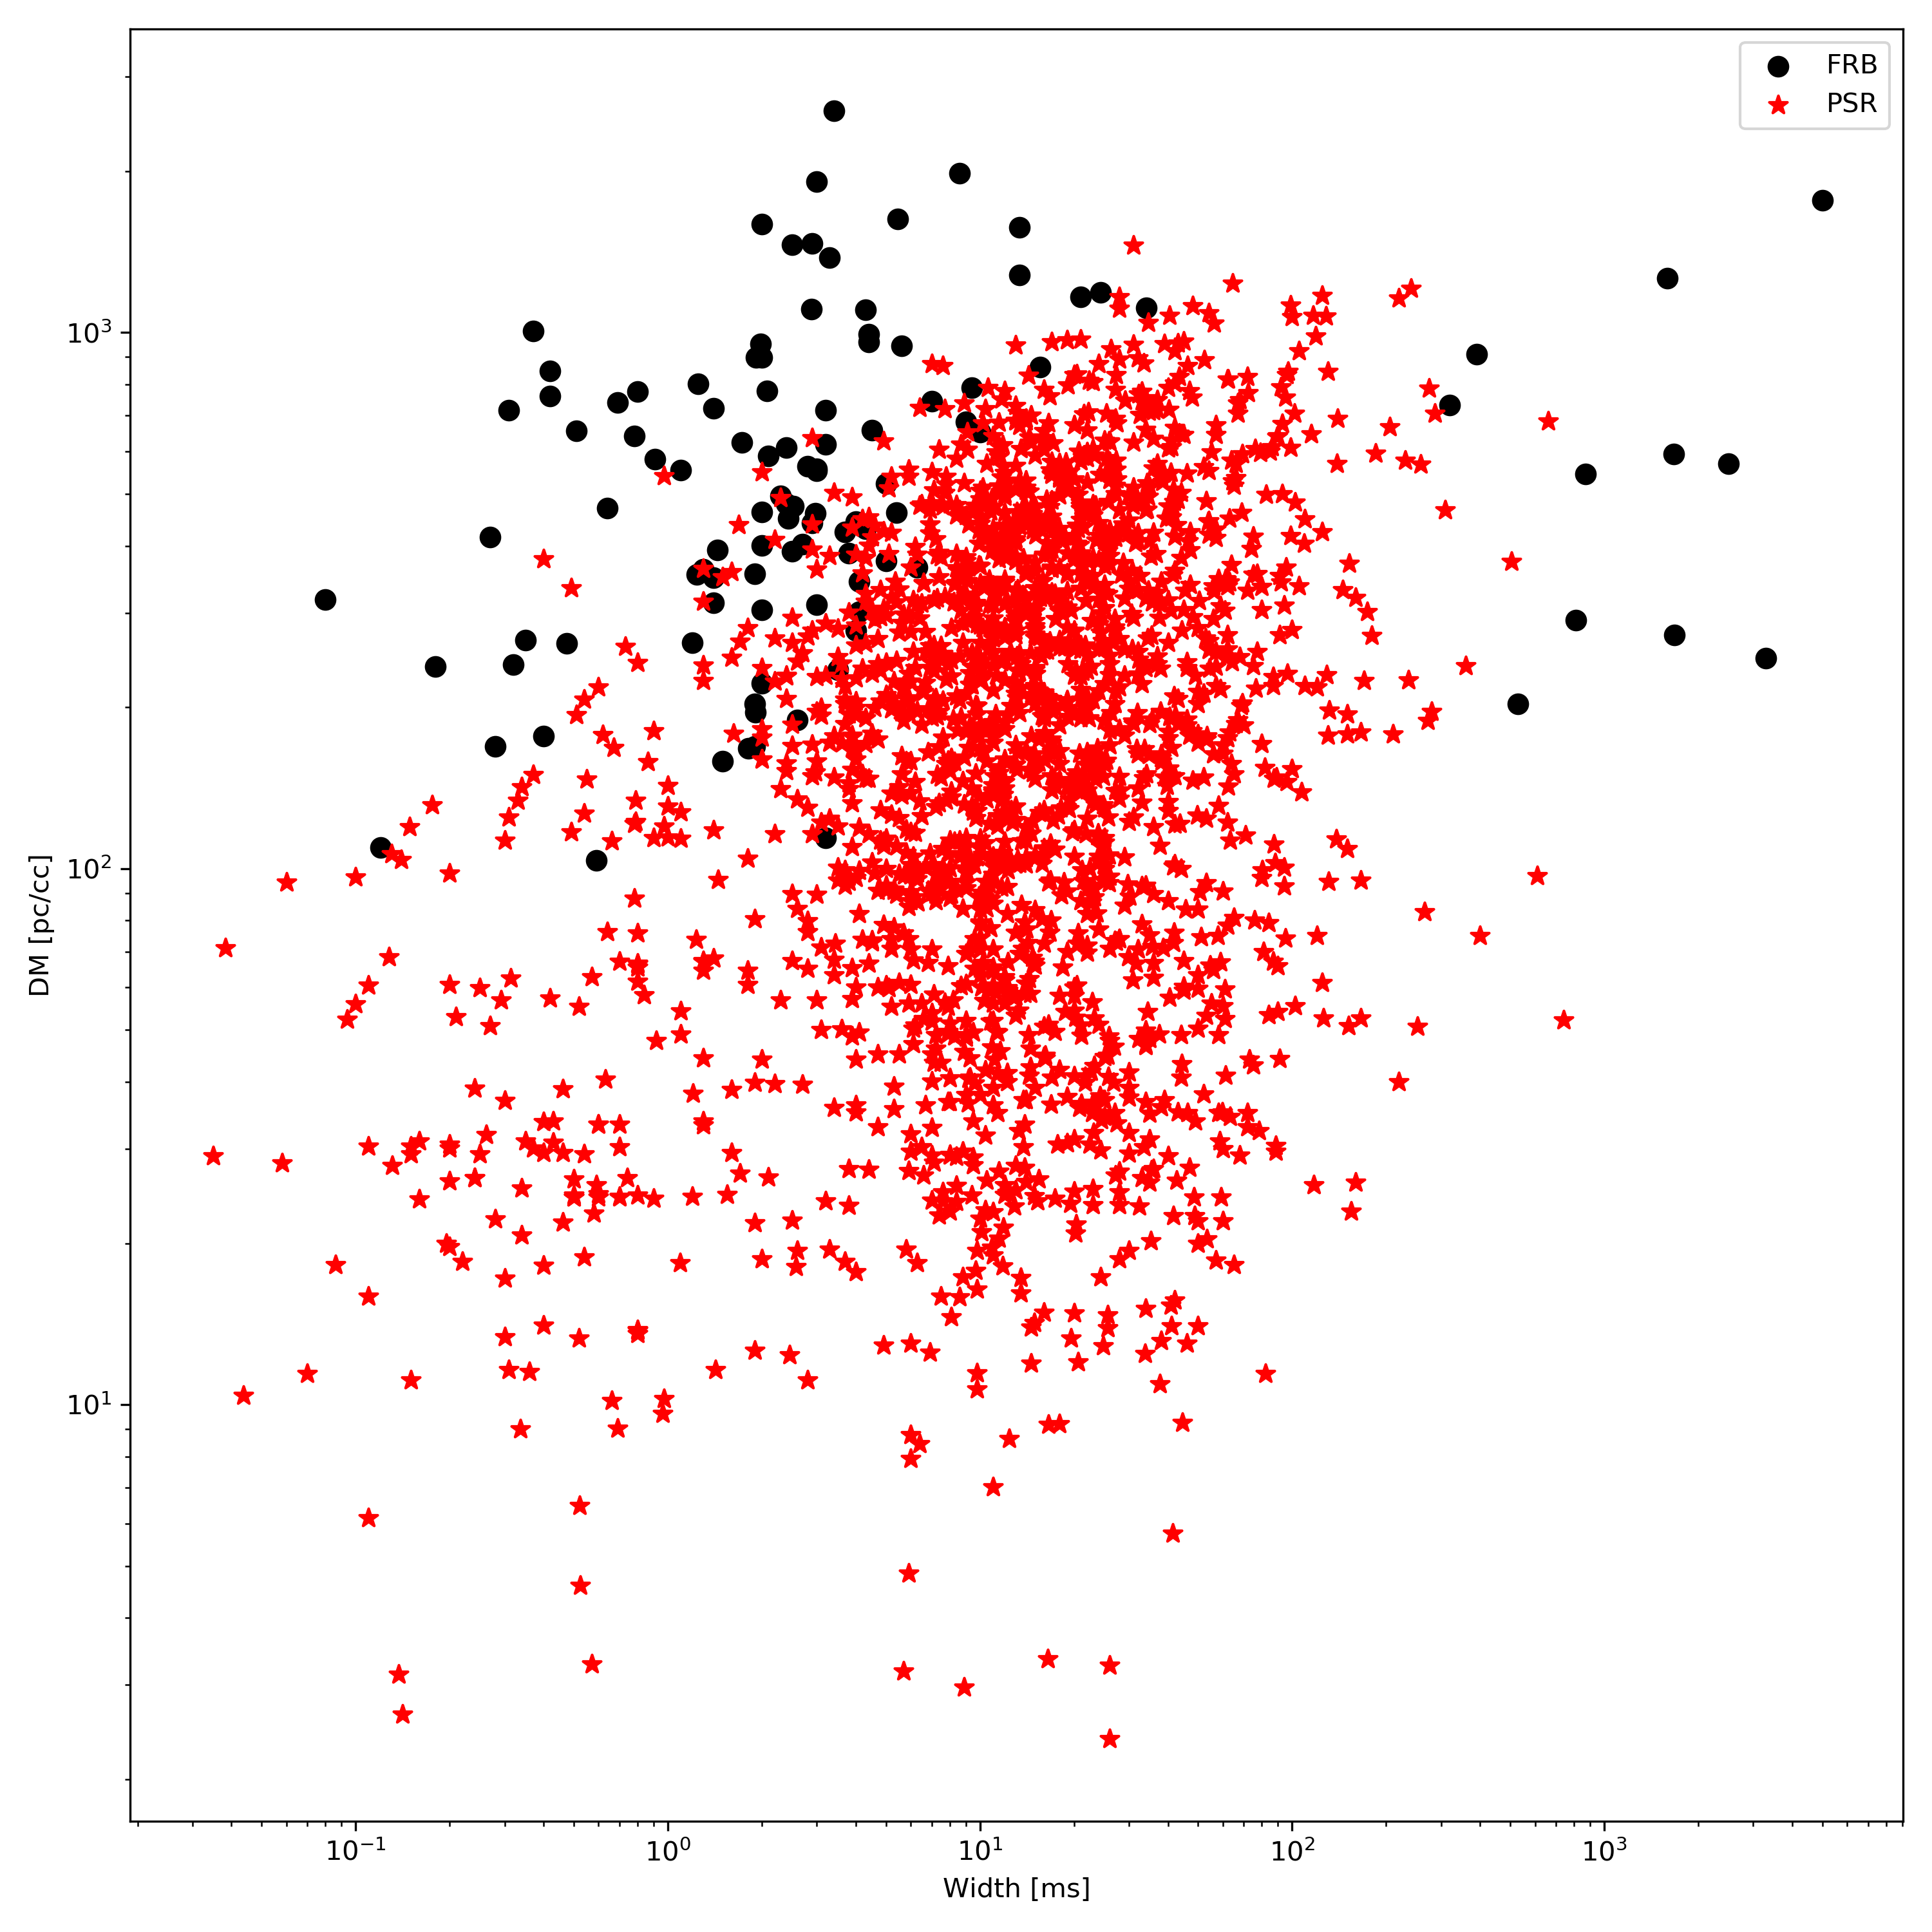
\includegraphics[width=0.8\textwidth,keepaspectratio]{frbpsr_scatter.png}
% \label{fig:scatter}
% \caption{PSRs and FRBs scatter plot of DM and Width}
% \end{figure}
% %% higher DM more reach final frontier is pushed further back
% \end{frame}

\begin{frame}
\begin{figure}
\centering
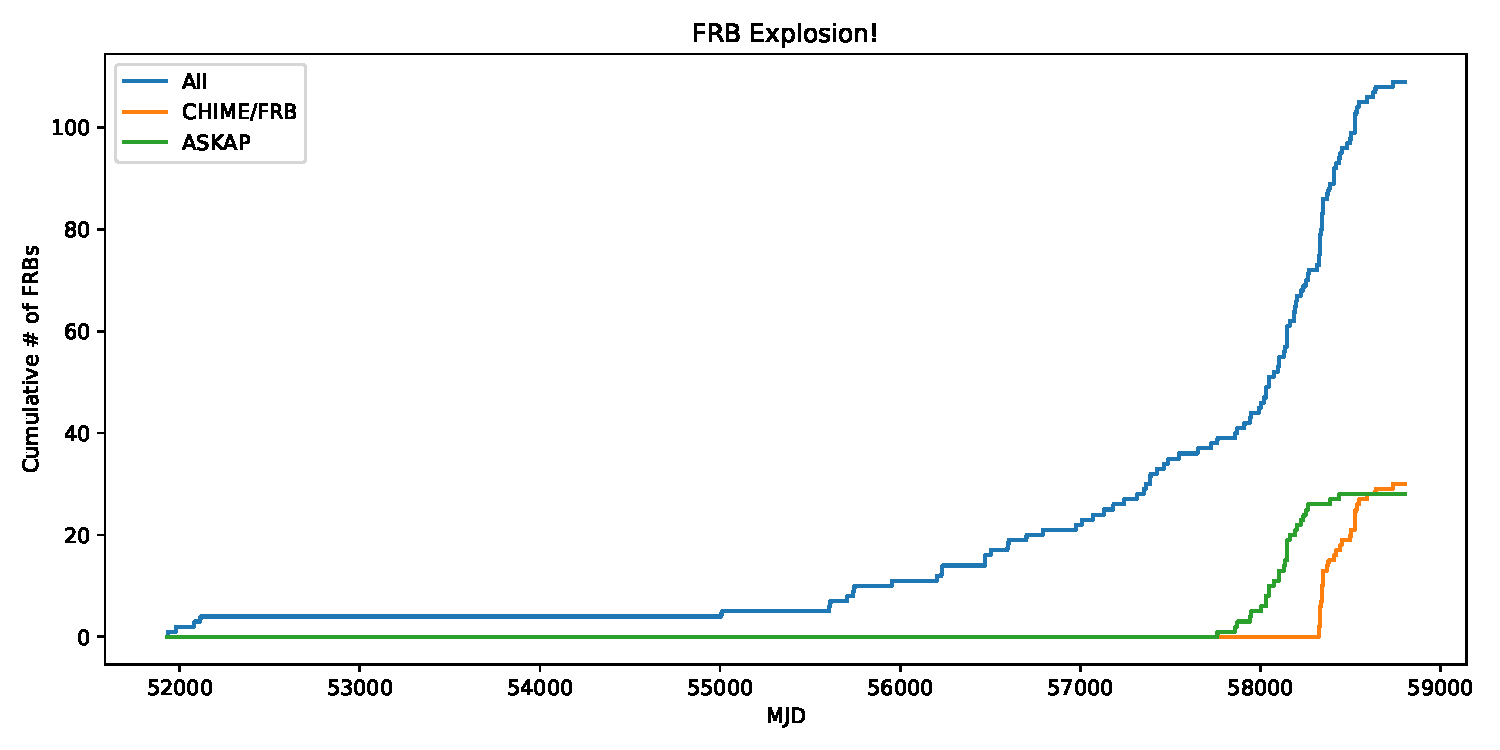
\includegraphics[width=\textwidth,keepaspectratio]{frbexplosion.pdf}
\label{fig:frbx}
\caption{Cumulative time plot. FRB explosion!}
\end{figure}
%% lot of research effort has already flown in. 
\end{frame}

